\section{Spatial discretization}
\label{sec:spat}
%
BOUT++ comes with a built-in set of spatial discretization operators.
The operators used in the CELMA code are given in \cref{tb:spatop}.
%
\begin{table}[h!]
{\footnotesize \centerline{
\colorme
\begin{tabular}{c|lll}
\hline\hline
%
Direction & First derivative stencil ($\partial_i f$) & Second derivative stencil ($\partial^2_i f$)& Upwind stencil ($f \partial_i g$)\\
%
\hline
%
$\rho$  & Centered second order & Centered second order & None\\
$\theta$ & Fast Fourier transform & Fast Fourier transform & None\\
z  & Centered second order & Centered second order & First order upwinding\\
%
\hline\hline
\end{tabular}
}}
\caption[]{\textit{Spatial operators used in the CELMA code.}}
\protect\label{tb:spatop}
\end{table}
%

\noindent
The standard centered finite difference stencils have been used (see \cite{Leveque2007book} for details).
Further, the fast Fourier transform is implemented using the \texttt{fftw}-package \cite{FFTW05}.
Finally, the first order upwinding scheme is used for the following operators:
%
\begin{itemize}[noitemsep]
    \item $u_{e,\|}\partial_\|\ln(n)$
    \item $nu_{e,\|}\partial_\| u_{i,\|}$
    \item $nu_{i,\|}\partial_\| u_{e,\|}$
    \item $\frac{j_{\|}}{n}\partial_\| u_{e,\|}$
    \item $u_{i,\|}\partial_\| \L(nu_{e,\|}\R)$
\end{itemize}
%
Note that whereas the upwinding makes the system more stable, it does so by introducing damping on the system through artificial numerical diffusion introduced by the discretization \cite{Leveque2007book}.
For this reason, upwinding is \textbf{NOT} used on the $u_{i,\|}\partial_\|\Om$ term when using the Boussinesq approximation as this may introduce spurious vorticity from the numerics.

\section{Boundary conditions}
%
The boundaries are positioned halfway between grid points, as depicted in \cref{fig:flatBC}.
%
\begin{figure}[htb]
    \centering
    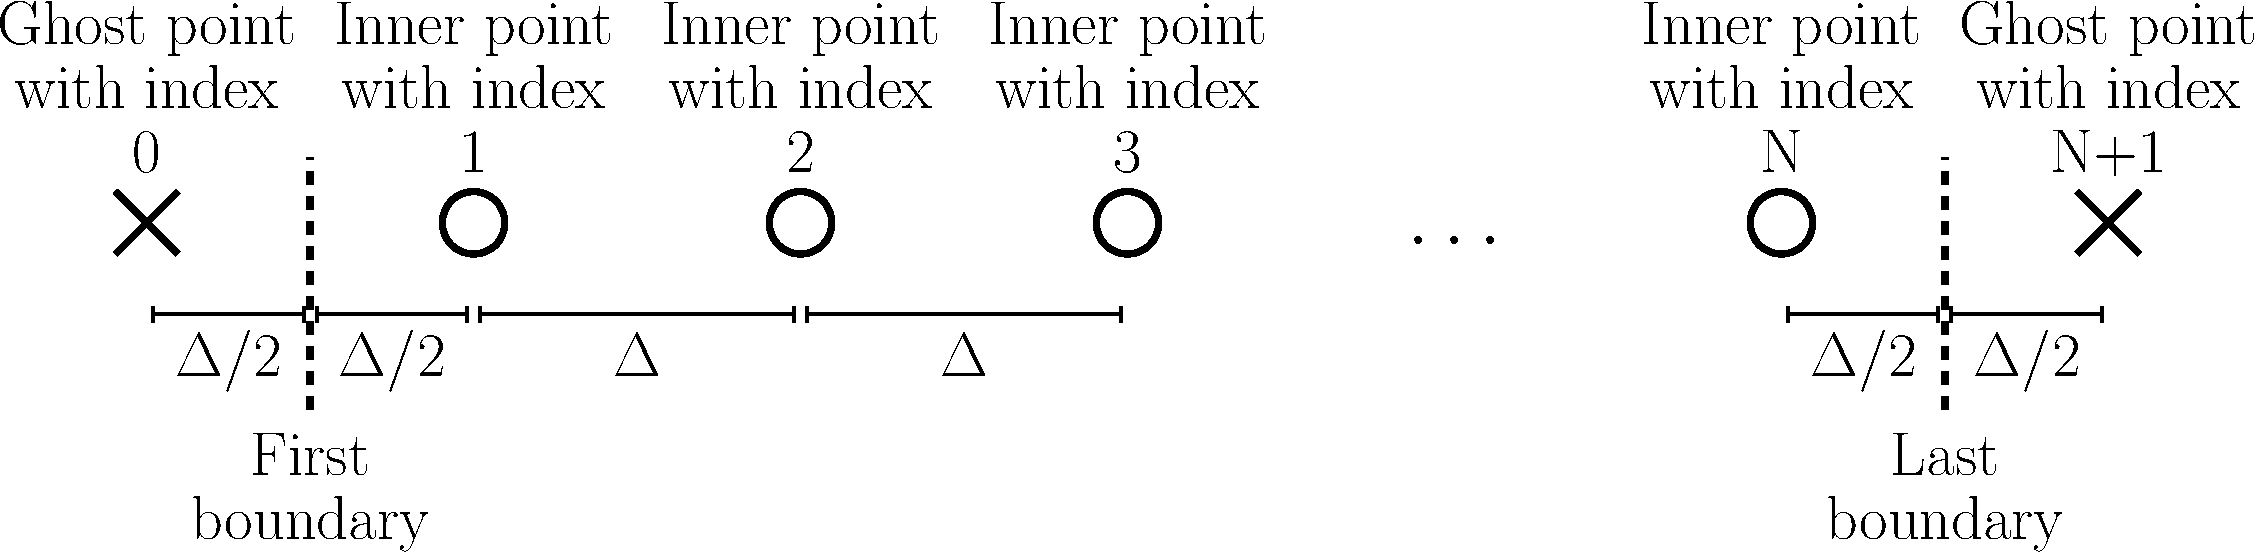
\includegraphics[width=1.0\textwidth]{fig/flatGrid}
    \caption{\textit{
            The boundaries are positioned halfway between grid points.
            $\Delta$ denotes the grid spacing between two grid points.
        }}
    \label{fig:flatBC}
\end{figure}
%

\noindent
The boundary conditions are specified at the position of the boundary (the dashed horizontal lines in \cref{fig:flatBC}).
As there is no grid point at the boundary, the value is extrapolated to the ghost point which is placed a distance $\Delta/2$ away from the boundary.
We will here specify how these extrapolations are done within the BOUT++ framework.
For implementation of artificial boundary conditions, see \cref{sec:extrapolGhost}.

For the Dirichlet boundary condition, the following \nth{4} order extrapolation%
%
\footnote{
    Derived using a Newton polynomial (using the four points around the edge of the domain of \cref{fig:flatBC} (including the ghost point)), evaluated in the ghost point.
} %
is used
%
\begin{align*}
      f_{0} =& \frac{16}{5}f_{\text{First boundary}}
              - 3          f_1
              +            f_2
              - \frac{1}{5}f_3
    \\
      f_{N} =& \frac{16}{5}f_{\text{Last boundary}}
              - 3          f_{N}
              +            f_{N-1}
              - \frac{1}{5}f_{N-2}.
\end{align*}
%
For the Neumann boundary condition, a \nth{4} order extrapolation%
%
\footnote{
    Derived using a one sided stencil (using the five points around the edge of the domain of \cref{fig:flatBC} (including the ghost point)) of the first derivative evaluated at the boundary, solved for the ghost point.
% See D4DX4/BW2ndOrderNeumann4thOrder
} %
%
is used, reading
%
\begin{align*}
      f_0 =& \frac{12}{11}\Delta f_{\text{First boundary}}
                +
                \frac{
                  17f_1
                +  9f_2
                -  5f_3
                +   f_4
               }{22}
    \\
      f_{N+1} =& \frac{12}{11}\Delta f_{\text{Last boundary}}
                +
                \frac{
                  17f_{N}
                +  9f_{N-1}
                -  5f_{N-2}
                +   f_{N-3}
               }{22}.
\end{align*}
%
Finally, as the $\theta$ direction is periodical, the ghost points are simply
%
\begin{align*}
    f_{N+1} =& f_{1}
    \\
    f_{0} =& f_{N}.
\end{align*}
